\section{SwitchBox Design}\label{sec:design}

\subsection{Quantifying the Security Dimension}

To reason about trading off the security guarantees provided by various ciphers,
the strength of these guarantees must be quantified through scoring. \TODO{We do
not want to say "For our purposes." We want to propose something that would be
useful for as many people as possible. Also, I want to be very careful about
attribution here. Is this scoring system all stuff you came up with? Did David
help at all? Is there anything here we can cite? Basically, if this is all
original work, then we should claim it as a contribution and argue that it is a
generally useful scheme. If some or all of it is prior work, that is fine, too,
we just need to attribute those pieces and make it clear that others have
already argued this is a useful way to compare ciphers. No matter what, we need
a stronger argument for this scheme than just that it serves our purposes.} For
our purposes, we consider three key features that, when scored, give us a useful
quantification of cipher security (see: \tblref{security-quant}).

\TODO{It might be worth talking about why it is hard to quantify security.
Maybe mention that if this is not your area, you might think it could be
quantified by the time to brute force, but there is more subtlety than that
including what assumptions you make about the attacker's access. }

\begin{itemize}

 \item \emph{Output randomization.} A cipher that exhibits output randomization
 can output ciphertext non-deterministically given the same input, which is
 extremely useful for FDE\@. This is a binary feature in that a cipher either
 outputs deterministically or it does not. A cipher with output randomization
 scores a 1 for this feature while a cipher without it scores a 0. \TODO{So, how
 does AES-XTS get a 0.2?}

 \item \emph{Resistance to cryptanalysis.} A cipher that is resistant to
 cryptanalysis can resist theoretical cryptanalytical attacks such as
 known-plaintext and chosen-plaintext attacks, offline key-guessing attacks, et
 cetera. Scores for this feature range from 0 to 1, where 0.5 represents
 standard resistance to cryptanalysis for stream ciphers in the general case\@.
 \TODO{Can we rename this feature? I feel like "resistance to cryptanalysis"
 should be equivalent to the overall cipher strength just going by the meaning
 of the words. Also, this bullet needs to be expanded more. Are these attacks
 a strict hierarchy, like if you are resistant to offline key-guessing attacks
 are you resistant to everything below that? Also, since this is a key point of
 the paper, we cannot just use et cetera, but we need to list all attacks we
 consider to arrive at this score. }

 \item \emph{Round count vs standard.} The ciphers we examine in this research
 are all constructed around the notion of \emph{rounds}, where a higher number
 of rounds implies a stronger confidentiality guarantee. This feature represents
 how many rounds the cipher executes compared to the accepted "standard" round
 count for that cipher. For instance, ChaCha8 is a reduced round version of the
 standard ChaCha20. Variants are distributed evenly from 0-1. For instance,
 ChaCha8 scores 0, ChaCha12 scores 0.5, and ChaCha20 scores 1\@. 

\end{itemize}

\TODO{It is very important that any reader who was sufficiently motivated could
follow the above bullets and arrive at the same values you have in this table.
If that is not the case, then we don't have a quantifiable metric of security as
much as a mapping of our own objective scores onto a number. For example,
Rabbit gets a CR of 0.4. I am not sure how that number is derived, but we have
to have a deterministic process so that everyone who applied it would arrive at
the same number. In general, I think this section just needs more detail. The
right level of detail is explain it so that anyone who read the section would
derive the same numbers that you have in this table.}

\begin{table}[]
  \begin{tabular}{@{}lllll@{}}
  \toprule
  \textbf{Cipher} & \textbf{OR} & \textbf{CR} & \textbf{RR/RK} & \textbf{Rank} \\ \midrule
  ChaCha8     & 0      & 0.5     & 0       & 0.5      \\
  ChaCha12    & 0      & 0.5     & 0.5      & 1       \\
  ChaCha20    & 0      & 0.5     & 1       & 1.5      \\
  Salsa8     & 0      & 0.4     & 0       & 0.4      \\
  Salsa12     & 0      & 0.4     & 0.5      & 0.9      \\
  Salsa20     & 0      & 0.4     & 1       & 1.4      \\
  AES128-CTR   & 0      & 0.5     & 0       & 0.5      \\
  AES256-CTR   & 0      & 0.5     & 1       & 1.5      \\
  HC128      & 0      & 0.5     & 0       & 0.5      \\
  HC256      & 0      & 0.5     & 1       & 1.5      \\
  Rabbit     & 0      & 0.4     & 1       & 1.4      \\
  Sosemanuk    & 0      & 0.4     & 1       & 1.4      \\
  Freestyle (F)  & 1      & 1      & 0       & 2       \\
  Freestyle (B)  & 1      & 1      & 0.5      & 2.5      \\
  Freestyle (S)  & 1      & 1      & 1       & 3       \\
  AES128-XTS   & 0.2     & 0.5     & 1       & 1.7
  \end{tabular}
  \caption{\TODO{Table caption goes here.}}
  \label{tbl:security-quant}
\end{table}

\PUNT{\begin{figure}[ht]
 \centering
 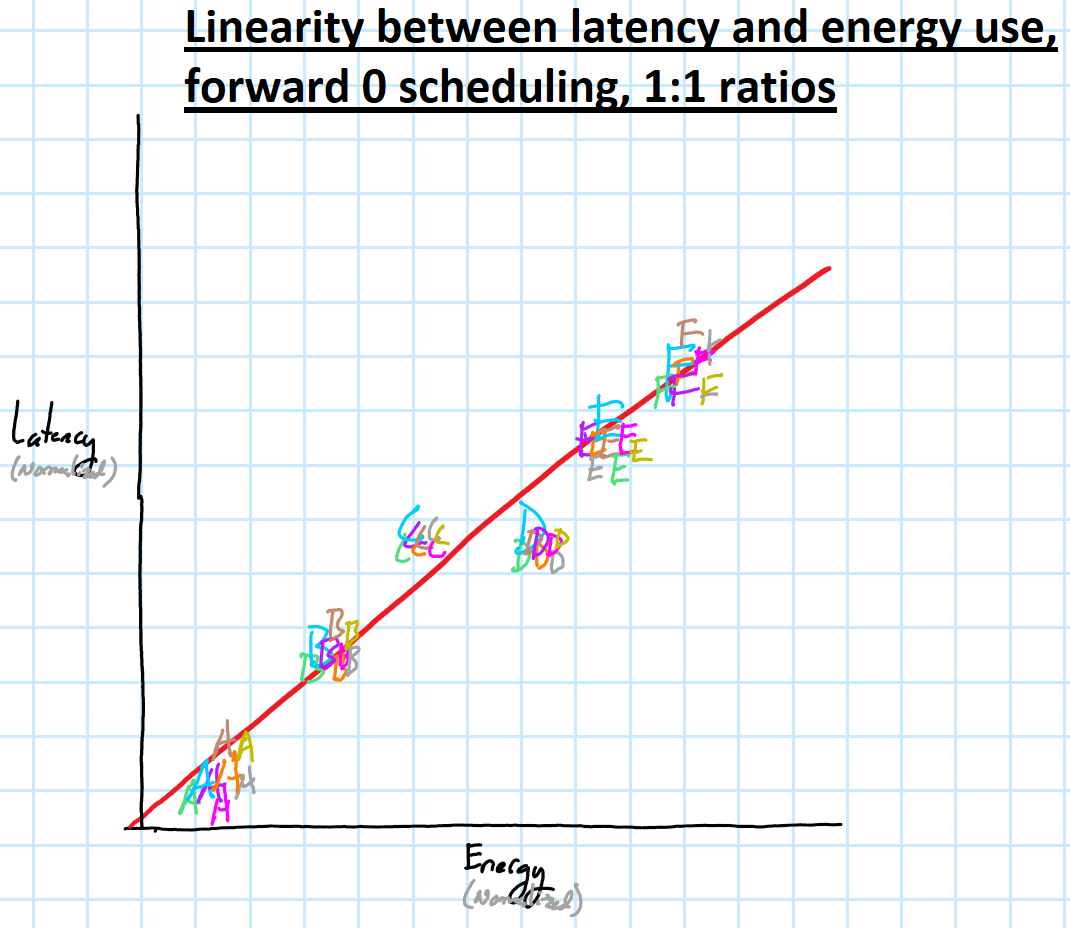
\includegraphics[width=\linewidth]{drawn/5.png}
  \caption{\TODO{Caption goes here}}\label{fig:energy-latency-linearity}
\end{figure}

\figref{energy-latency-linearity} shows that, for the stream ciphers included in
our experiments, there is a linear relationship between cipher performance and
total energy used during the I/O operation.

With prior work, \TODO{we could cite other filesystems and storage layers here
other than just StrongBox, such as ZFS, dmcrypt?} cipher configuration is made
statically at compile time or at filesystem initialization. This static choice
forces developers and end-users to choose a configuration that works best in the
most general case and stick with it, even if a different configuration becomes
more optimal at a later point. The only way to switch ciphers when a new
configuration becomes more optimal is to recreate the entire underlying
filesystem, which is rarely desirable. \TODO{This paragraph should be fleshed
out more?} \TODO{Yes, please do flesh it out more. Add the citations you
suggested. I think you should start with the good thing: different ciphers have
a wide range of energy/latency vs security properties. Then you can highlight
the two key drawbacks (maybe even bullet-point them): (1) They don't actually
form a continous tradeoff space, but represent discrete points, and what if you
need to be in the middle? and (2) They are fixed by the time the system finishes
booting (?) and if requirements change online the system requires a reboot.}}

\begin{figure}[t]
   \centering
   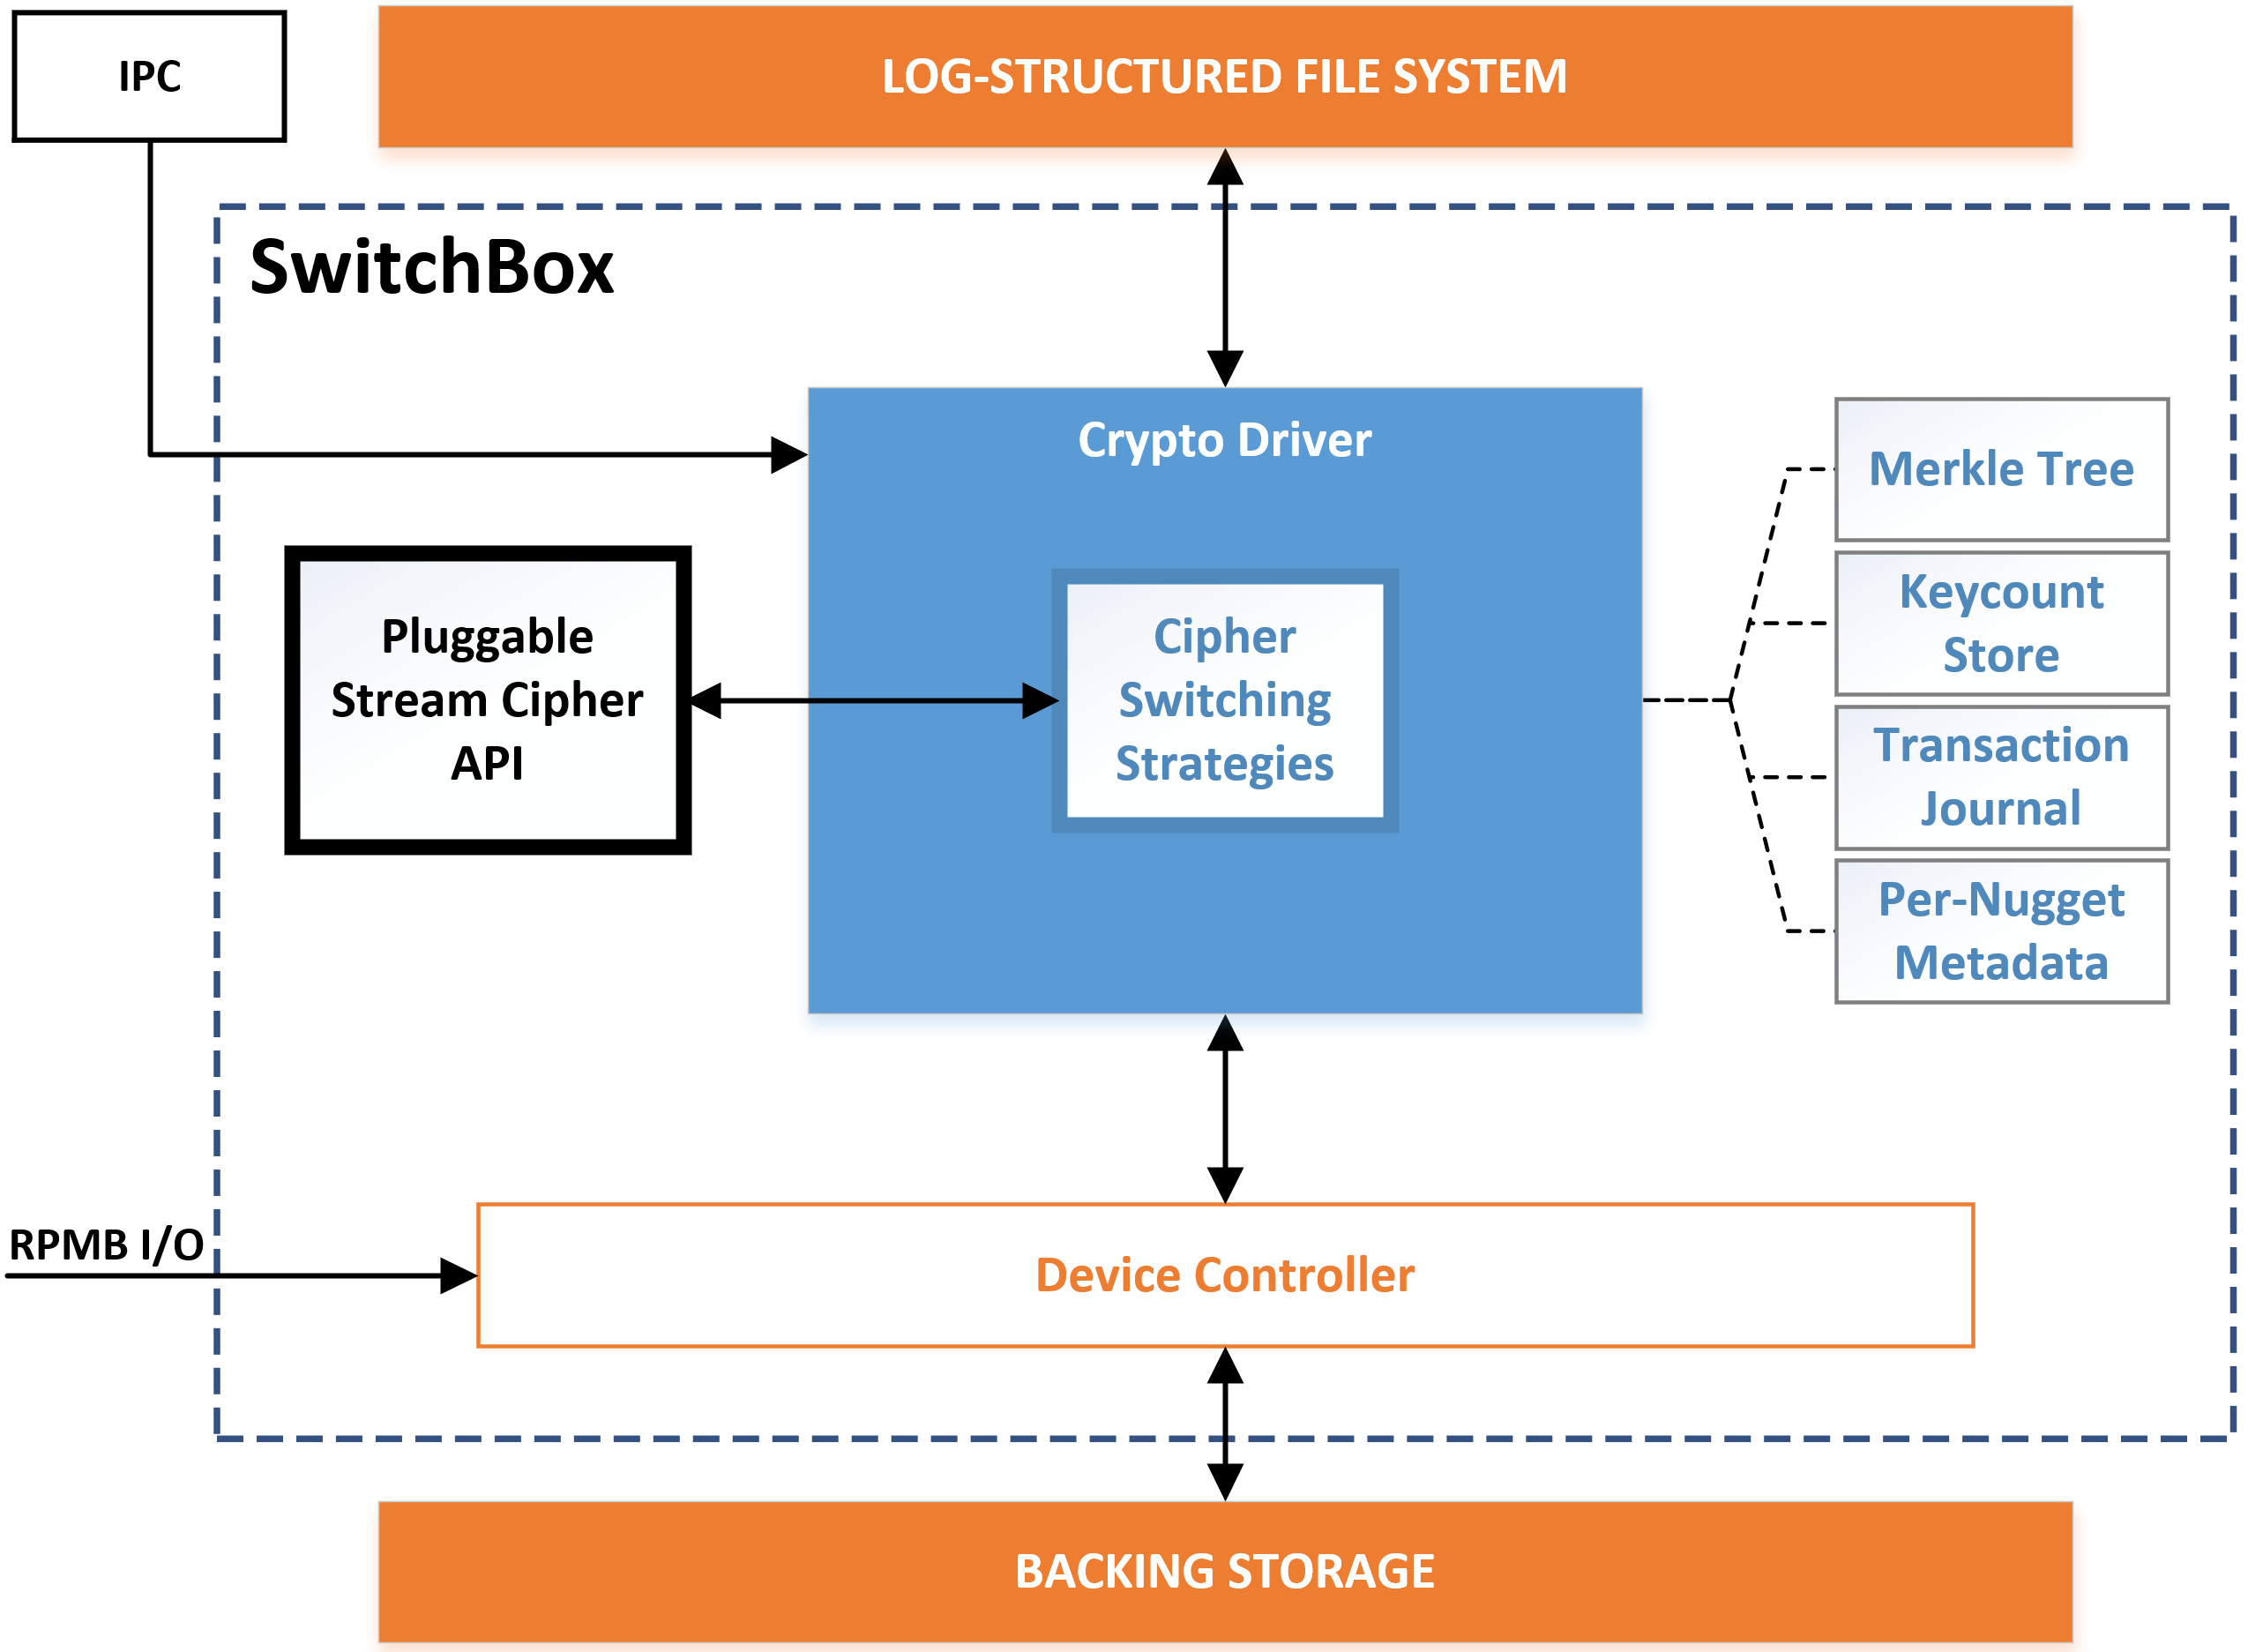
\includegraphics[width=\linewidth]{overview.png}
    \caption{Overview of the SwitchBox construction.}\label{fig:overview}
  \end{figure}

SwitchBox, like StrongBox and Adiantum, is a translation layer positioned
between the block layer and the operating system's virtual file
system~\cite{StrongBox}. There are several places SwitchBox could be implemented
in the system stack: as part of an actual kernel Log-structured File System
(LFS) module like the F2FS filesystem, as a block device or virtual block device
in the manner of dm-crypt, or within a device controller such as an SSD drive
controller's FTL~\cite{StrongBox}.

\figref{overview} illustrates the SwitchBox design. SwitchBox manages five
metadata components: an in-memory \emph{Merkle Tree}; two drive-backed byte
arrays, \ie{the \emph{Keycount Store} and the \emph{Transaction Journal}}; a
globally persistent cryptographically secure monotonic counter; and a flexible
drive-backed store for per-nugget cipher-specific metadata. For our monotonic
counter implementation, we used a \emph{Replay Protected Memory Block} (RPMB).
\TODO{Citation would be good here. But, it is a little strange to get so
specific in this part of the text. I would either save it for a later
implementation section (or evaluation). Or, if you think that the existence of
these counters might be controversial, then say we use RPMB, but we could have
used many others such as...}

These five components are tightly integrated into the cryptographic driver,
which handles data encryption, decryption, overwrite detection, integrity
protection, communication with the wider system to determine the active cipher,
and the application of cipher switching strategies. The cryptographic driver
interacts with 1) the overlying LFS through traditional I/O passed through the
Linux Virtual Filesystem Switch (VFS) as well as 2) the underlying backing store
through the device controller block I/O layer.

SwitchBox uses IPC to receive commands to toggle the active cipher between the
primary and secondary ciphers. \TODO{Spell out the acronym the first time it is
used.}

\begin{figure}[t]
 \centering
 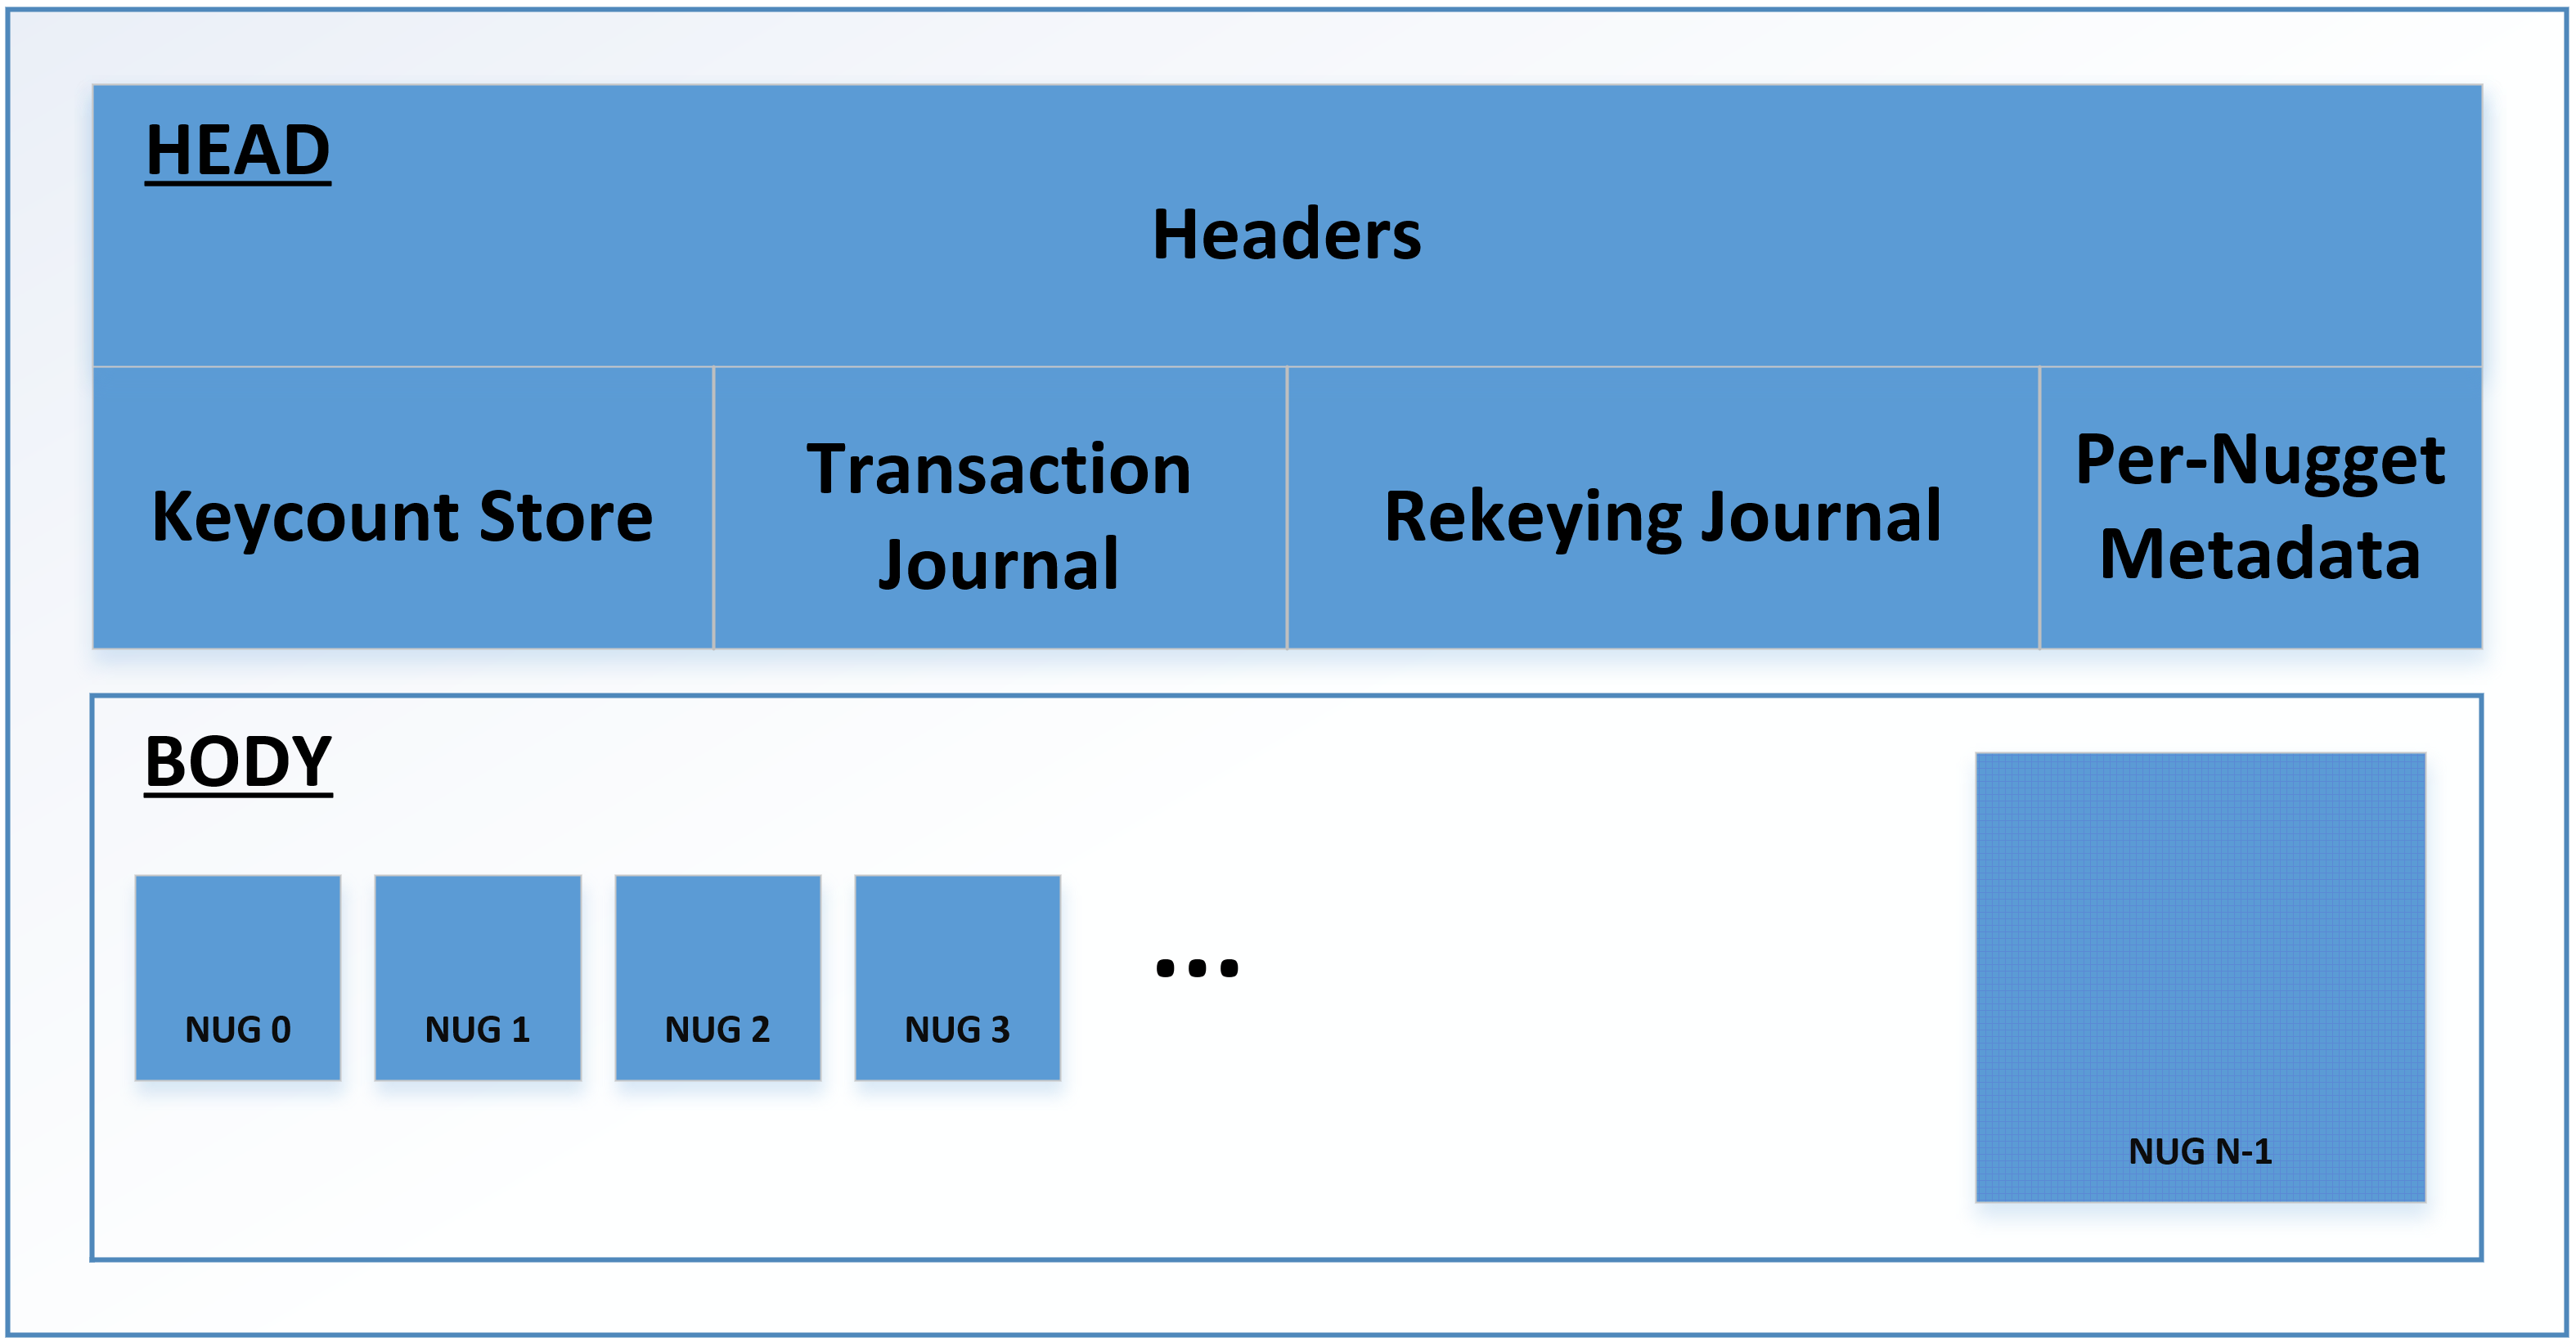
\includegraphics[width=\linewidth]{backstore.png}
  \caption{Layout of SwitchBox's backing storage.}\label{fig:backstore2}
\end{figure}

The backing store is the storage medium SwitchBox operates on. The layout of the
backing store is illustrated in \figref{backstore2}. In the \textit{body} section
of the backing store layout, end-user data is partitioned into a series of
same-size \emph{logical blocks}---which are distinct from the concept of
\emph{physical drive blocks}---we refer to these wider logical blocks as
\emph{nuggets}, marked \textit{NUG}. Hence, a nugget consists of one or more
physical drive blocks along with per-nugget metadata indicating if the nugget
was encrypted with the primary or the secondary cipher. \TODO{Do we redescribe
the rest of the backing store from StrongBox, or should we link to the original
paper? Or should we skip talking about the backing store at all and more briefly
describe nuggets here? It's all not very different from StrongBox's, i.e. an
extra header was added.}

In the rest of this section, we describe our cipher switching strategies. We
also discuss the pluggable stream cipher API and other design challenges. This
is followed by an explanation of implementation-specific details and a
discussion of the overall implications and limitations of SwitchBox's design.

\subsection{Cipher Switching Strategies}

Upon initialization, prior work requires a single cipher to be selected. The
specified cipher---ideally along the pareto frontier of security and energy
tradeoffs---is then used to encrypt and decrypt all data on the filesystem. With
SwitchBox, however, \emph{a pair of ciphers are selected} upon initialization,
depending on the concerns of the end-user. These ciphers are referred to as the
\emph{primary cipher} and the \emph{secondary cipher} respectively, and
represent the static configuration points along the pareto frontier between
which SwitchBox can navigate. \TODO{Do you really have to know these ahead of
time? If I had a cipher API and managed the implementation as a DLL, could I
switch to any cipher, by just building a new DLL? Is there any reason, you
couldn't have three or four or N ciphers and switch between all of them? I ask
all these questions because I want you to separate the conceptual idea, which
should be as broad as possible, from the specific choices you had to make to
demonstrate the idea (which may be much more restricted). Here we want to
discuss the conceptual ideas and save details for the implementation.}

At any moment, the currently active cipher is used to interact with the backing
store. Initially, the primary cipher is the active cipher. Until the wider
system indicates that SwitchBox should use a different cipher to interact with
the backing store, SwitchBox functions identically to StrongBox in that it uses
the primary cipher to encrypt and decrypt all nuggets during I/O.

However, switching the active cipher dynamically allows SwitchBox to achieve
optimal configuration points that are otherwise unachievable with prior work.
The wider system determines if the primary or secondary cipher should be the
active cipher at any given moment, and SwitchBox responds immediately.
Unfortunately, it is entirely non-trivial to determine \emph{when} to re-encrypt
a nugget with a different cipher and \emph{where} to direct the output of that
cipher. \TODO{Don't just say it is difficult, make an argument about why it is
difficult. It is often very helpful to say things that are obvious to you
because they won't be obvious to the reader, but will help build intuition for
what is coming. For example, you can say that one simple approach would
immediately convert the entire drive, but the cost of doing that conversion
might consume more energy than would be saved in future accesses. I do like
using where and when to set up spatial and temporal switching. }

Hence, cipher switching \emph{strategies} are the mechanism by which SwitchBox
can effectively transition nuggets between different encrypted states
dynamically, thus providing a mechanism to navigate the tradeoff space presented
in \figref{40mb-read-with-forward}. \TODO{Expound on this all more? Reword?
Delete? Different chart referenced here instead?} \TODO{Hank: expound! Go ahead
and say that when to target the new encryption is temporal switching and we
propose a specific strategy, \emph{Forward}, to handle it. Where to switch is
spatial switching and we propose two strategies to deal with that.}

\subsubsection{Forward Switching Strategy}

SwitchBox allows each individual nugget to exist encrypted using one cipher or
the other regardless of the currently active cipher. When a nugget is
encountered during I/O that is encrypted using a cipher other than the active
cipher, however, the forward strategy dictates that this nugget be re-encrypted
"just-in-time" using the active cipher before completing the I/O operation. If a
particular nugget encrypted with the non-active cipher is never encountered
during I/O, it is never re-encrypted and remains on the backing store in its
original state. In this way, the forward strategy represents a form of temporal
cipher switching.

Rather than re-encrypt the entire backing store every time the active cipher
changes, this strategy limits the performance impact of cipher switching to
individual nuggets. Similar to rekeying in the original StrongBox construction,
the heavy price of re-encryption is paid only once during the initial
re-encryption, after which the nugget is accessed normally during I/O until the
active cipher is switched again.

There are several forms the forward strategy can take. The default and most
intuitive is \emph{0-forward}, in which SwitchBox immediately transitions
individual nuggets encountered during I/O to the active cipher is they are not
using it. Over time, if various I/O operations end up touching every nugget in
the backing store, the encrypted state of every nugget will eventually become
consistent with the currently active cipher.

The forward strategy can also take the form of \emph{N-forward}, where SwitchBox
attempts to take advantage of spatial sequential locality to transition whole
sets of nuggets into the active cipher. We can trivially expand the forward
strategy to encompass the entire backing store by selecting N equal to the total
number of nuggets managed by SwitchBox. This would have the overhead of
re-encrypting large swaths of the backing store upon every I/O operation where a
nugget encrypted with the non-active cipher is encountered. Of course, this has
the same effect as simply re-initializing the entire filesystem with the new
cipher.

\subsubsection{Selective Switching Strategy}

When SwitchBox is initialized with the selective strategy, the backing store is
partitioned into two regions governed exclusively by the primary and secondary
ciphers, respectively. All nuggets in the first partition are encrypted with the
primary cipher while all nuggets in the second partition are encrypted with the
secondary cipher.

Hence, unlike the forward strategy, which schedules individual nuggets to be
re-encrypted at some point in time \emph{after} the active cipher is switched,
the selective strategy allows the wider system to indicate \emph{where} on the
backing store a read or write operation should occur: either in one partition or
the other. In this way, the selective strategy represents a form of spatial
cipher switching where different regions of the backing store can store
different pieces of data.

\subsubsection{Mirrored Switching Strategy}

Similar to the selective strategy, when SwitchBox is initialized with the
mirrored strategy, the backing store is partitioned into two regions governed
exclusively by the primary and secondary ciphers, respectively. All nuggets in
the first partition are encrypted with the primary cipher while all nuggets in
the second partition are encrypted with the secondary cipher.

However, unlike the selective strategy, all write operations that hit one
partition are mirrored into the other partition immediately. The mirrored
strategy allows the wider system to indicate where on the backing store a
\emph{read} operation should occur. As a result, both regions of the backing
store will always be in a consistent state and share the same data. In this way,
the mirrored strategy, like the selective strategy, represents a form of spatial
cipher switching.

\subsection{Pluggable Stream Cipher API}

\TODO{Always use present tense in technical writing. It should be we develop
instead of we developed.} We developed an API to allow any stream cipher or any
cipher that can pose as a stream cipher to be used with SwitchBox without
modification, including ciphers with residual output, \eg{Freestyle}. \TODO{I
don't know what residual output is, so please expand on the differences between
ciphers that causes problems. But before you do, see the note below on
challenges.} SwitchBox exposes a common encryption and decryption interface,
including read and write handles, that allow SwitchBox to transition nuggets
between arbitrary ciphers at the behest of the wider system. \TODO{This section
is odd here. Having a whole subsection seems to imply that it is as important
as the switching strategies, but having a short paragraph implies it is more of
a side note. In addition, it is not clear what purpose this discussion serves.
I think you need more setup about how different stream ciphers might appear to
all be interchangeable, but they are not, so we need a common interface---again,
sometimes it is actually helpful to state what feels obvious to you.}

\subsection{Additional Challenge: Beware Naive Forward Switching}

It is tempting to implement forward switching such that a nugget is re-encrypted
during I/O if its metadata indicates that it was previously encrypted using the
non-active cipher. However, such a naive implementation can have disastrous
effects on performance depending on the workload.

First, a nugget is considered "pristine" if it has not had any data written into
it yet. SwitchBox determines if a nugget is pristine by checking the state of
the transaction journal for that nugget. A pristine nugget will have a clean
transaction journal.

All nuggets start out as pristine. All nuggets start out with metadata
indicating that they're to be encrypted and decrypted by the primary cipher
(which is the initially active cipher when SwitchBox is first initialized). This
is true \emph{even if the nugget has not been written to yet}. This means, on
read and write operations after the secondary cipher becomes the active cipher
using a naively implemented forward switching strategy, every write operation
will trigger a re-keying, which carries significant overhead.

The solution is to divide forward switching into \emph{soft re-encryption} and
\emph{hard re-encryption}. Fortunately, the SwitchBox design lends itself nicely
to such a distinction for free, as per-nugget metadata is managed separately
from a nugget's actual data.

During soft re-encryption, only the nugget's metadata is changed to indicate
that the nugget can be encrypted and decrypted with the newly active cipher but
\emph{without actually re-encrypting the nugget data itself}. This keeps the
nugget in a "pristine" condition, preserving SwitchBox's ability to write data
into it without triggering a costly rekeying operation every time, preserving
the original StrongBox's performance advantage. At the same time, SwitchBox can
now use the newly active cipher to interact with the nugget as expected.

On the other hand, during hard re-encryption, the nugget's metadata is changed
to match the active cipher \emph{and} the nugget data is re-encrypted using the
new cipher. When using forward switching other that 0-forward, \ie{N-forward}
where $N > 0$, only read operations are allowed to trigger hard re-encryption
for nuggets other than the currently active nugget. This is still not enough to
preserve StrongBox's performance advantage, however, as I/O operations can span
multiple nuggets, and attempting to take advantage of spatial locality after
interacting with every nugget is counterproductive. Hence, only the last nugget
touched by a read or write operation will trigger the more aggressive N-forward
behavior if $N > 0$.

These considerations have the effect of 1) preserving the original StrongBox
performance advantage over prior work and 2) allowing more aggressive N-forward
behavior (where $N > 0$) to take advantage of spatial locality during read-heavy
workloads to result in a further performance advantage (c.f.
\secref{evaluation}).

\subsection{Threat Models}

\TODO{Hank: I feel like we need some discussion of threat model or something.
For example, I really like the mirroring strategy, but I think it breaks if an
attacker has physical access to the drive, right? Like if they have to request
IO through the OS, I think it works becuase the os or hypervisor can hide the
mirrored side, but you can't hide that if I can just read bytes off the drive
itself, right? Sort of similar for forward. We really do need to say something
about when these are applicable and when they aren't.}
